\documentclass[]{scrreprt}
\usepackage[utf8]{inputenc}
\usepackage[T1]{fontenc}
\usepackage[a4paper , tmargin=1cm, lmargin=2cm, rmargin=2cm]{geometry}
\usepackage[french]{babel}
\usepackage{graphicx}
\usepackage{listings}
\usepackage{xcolor}
\usepackage{amssymb}
\usepackage{amsmath}
\usepackage{mathrsfs}
\usepackage{tcolorbox}
\usepackage{tikz}

\usepackage{tcolorbox}
\tcbuselibrary{theorems}

\usepackage[backend=biber]{biblatex}
\usepackage{csquotes}
\usepackage[colorlinks=true,urlcolor=blue,linkcolor=black]{hyperref}

\newsavebox{\tempbox}
\newenvironment{definition}{
	\begin{lrbox}{\tempbox}
		\begin{minipage}{\textwidth}
		}{
		\end{minipage}
	\end{lrbox}
	\begin{center}
		\fcolorbox[HTML]{222222}{EEEEEE}{
			\usebox{\tempbox}
		}
	\end{center}
}

\newcommand{\emf}[1]{\textbf{#1}}
\title{Projet Base De Données}
\subtitle{L2 Double Licence Mathématiques-Informatique}
\author{El houfi Othman \\ Benamara Abdelkader Chihab}


\begin{document}
	\makeatletter
	\begin{titlepage}
		\begin{center}
			
\includegraphics[scale=0.3]{logo-up7d.png}\\[4ex]\vspace{2cm}
			{\huge \bfseries  \@title }\\[2ex]\vspace{0.5cm}
			{\large  \@subtitle }\\[10ex] \vspace{2cm}
			{\large  \@author}\\[50ex] 
			{\large \@date}
		\end{center}
	\end{titlepage}
	\makeatother
	
	\tableofcontents
	
	\chapter{Introduction}
	\label{Chapter1}
	
		{\large Commençant par expliquer la problématique qui était posée dans le sujet. Après une perte d’informations dans les serveurs des Jeux Olympiques, on nous a chargé de mettre au point le plus rapidement possible une base de données concernant les Jeux Olympiques de l’été 2016, à Rio.\\
		Cette base de données dois contenir les athlètes qui participent à Rio, et les informations associées à ces athlètes (sexe, date de naissance, médaille ...), ainsi de distinguer ceux qui jouent individuellement et ceux qui jouent en équipes, sans oublié les épreuves voire les sous-épreuves joué par chaque athlète.\\
		Ce rapport contiendra plus de détails sur chaque étape ainsi qu’une explication logique derrière chaque décision prise lors traitement de cette problématique.}
		

	\chapter{Modélisation}
	\label{Chapter2}
	
		\begin{center}
			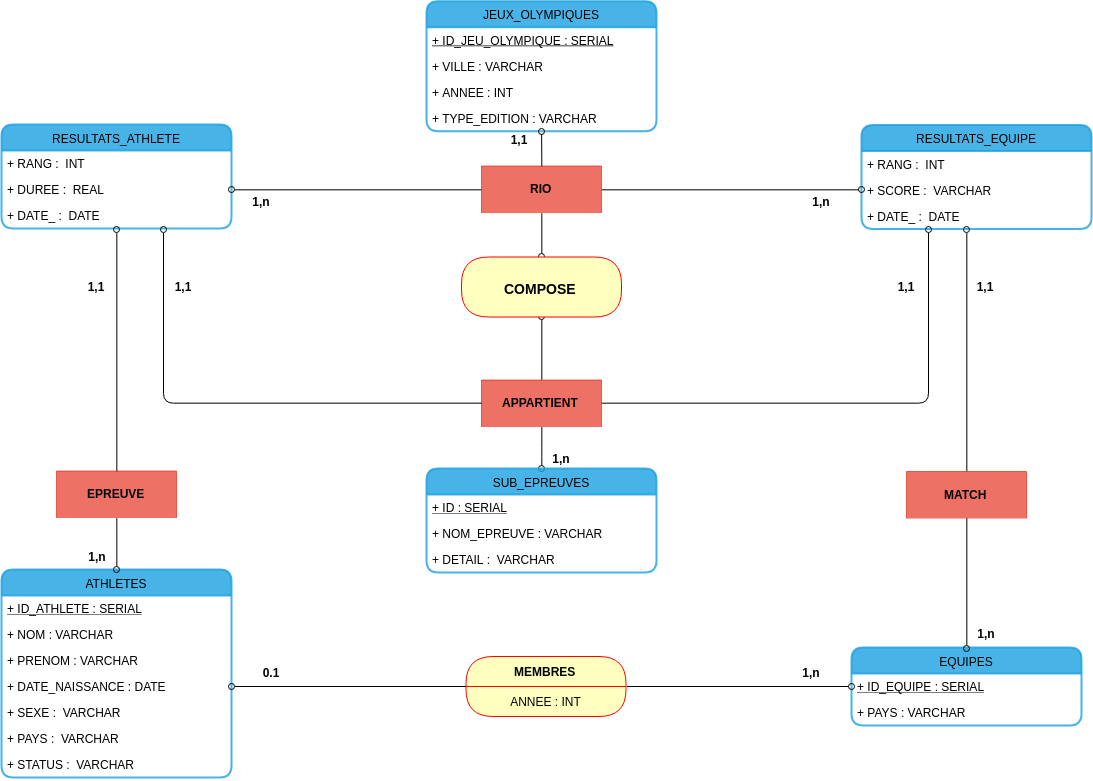
\includegraphics[scale=0.56 , angle=270]{DiagramAlpha.png}
		\end{center}	
	
	\chapter{Créations}
	\label{Chapter3}
	
		\section{Descriptions des tableaux}
		
		
		\newtcbtheorem[]{mytheo}{Tableau}
		{colback=green!5,colframe=red!35!black,fonttitle=\slshape}{th}
		
			\vspace{1cm}
	
			\begin{mytheo}{JEUX\_OLYMPIQUES}{}
				Contient la ville et l'année où se déroule les jeux olympiques, ainsi que leurs types (Hiver ou Été).
			\end{mytheo}
			
			\vspace{0.5cm}
			
			\begin{mytheo}{EPREUVES}{}
				Contient le nom des sport et leurs catégorie (Équipe ou Individuelle)(Ce tableau n'est pas nécessaire).
			\end{mytheo}
		
			\vspace{0.5cm}
			
			\begin{mytheo}{SUB\_EPREUVES}{}
				Contient les sous épreuves de chaque sport.
			\end{mytheo}
		
			\vspace{0.5cm}
			
			\begin{mytheo}{ATHLETES}{}
				Contient les détails de chaque athlète (nom, prénom, date de naissance, sexe, pays), ainsi que la catégorie de sports dont il participe (Équipe ou Individuelle).\\
				Attention : Dans ce projet on a pas pris en considération les athlètes qui jouent individuellement et en même temps en équipe car on a peuplé les tables automatiquement grâce à un script python et cela exclu le cas précèdent. 
			\end{mytheo}
		
			\vspace{0.5cm}
			
			\begin{mytheo}{COMPOSE}{}
				Contient les sous épreuves qui existent dans chaque édition des jeux olympiques.
			\end{mytheo}
		
			\vspace{0.5cm}
			
			\begin{mytheo}{EQUIPES}{}
				Contient les équipes de chaque pays et leur sous épreuve.
			\end{mytheo}
			
			\vspace{0.5cm}
			
			\begin{mytheo}{MEMBRES}{}
				Contient les athlètes de chaque équipe.
			\end{mytheo}
			
			\vspace{0.5cm}
			
			\begin{mytheo}{RESULTATS\_ATHLETE}{}
				Décrit l'état de chaque athlète, les médailles gagnées par cette athlète (Rang), dans quelle sous épreuve, dans quel jeux olympiques, ainsi que la date où elle a reçu cette médailles, voire d'autre détails (Durée) .\\
				Rang=1 (Médaille d'or).\\
				Rang=2 (Médaille d'argent).\\
				Rang=3 (Médaille de bronze).\\
				Rang>3 (Aucune médaille).
			\end{mytheo}
			
			\vspace{0.5cm}
			
			\begin{mytheo}{RESULTATS\_EQUIPE}{}
				Décrit l'état de chaque équipe, les médailles gagnées par cette équipe (Rang), dans quelle sous épreuve, dans quel jeux olympiques, ainsi que la date où elle a reçu cette médailles, voire d'autre détails (Score) .
			\end{mytheo}
			
			\vspace{0.5cm}
		
		
		
		\section{Requêtes de Créations}

			
			{\large Dans cette partie on a traduit notre schéma qui modélise l’architecture de notre base de données à des requêtes SQL afin de créer les tableaux nécessaires ainsi que les relations et les contraintes liées à chaque tableau.}
			
			{\footnotesize 
				\begin{verbatim}
			
				=======================  CREATION_JEUX_OLYMPIQUES  =======================
				
				CREATE TABLE IF NOT EXISTS JEUX_OLYMPIQUES
				(
				ID_JEU_OLYMPIQUE      serial NOT NULL,
				VILLE                 VARCHAR(30),
				ANNEE                 int,
				TYPE_EDITION          VARCHAR(10),
				CONSTRAINT PK_JEUx_OLYMPIQUEs PRIMARY KEY (ID_JEU_OLYMPIQUE),
				CONSTRAINT CK_VILLE_JEUX_OLYMPIQUES CHECK (VILLE IS NOT NULL),
				CONSTRAINT CK_VALIDITE_DATE CHECK ( (TYPE_EDITION = 'ETE' AND MOD((ANNEE - 1912),4) = 0) 
					OR  (TYPE_EDITION = 'HIVER' AND MOD((ANNEE - 1994),4) = 0 ) )
				);
				
				\end{verbatim}}
		
			{\footnotesize 
			\begin{verbatim}
			
			=======================  CREATION_EPREUVES  =======================
			
			CREATE TABLE IF NOT EXISTS EPREUVES
			(
			NOM_EPREUVE      VARCHAR(100),
			TYPE_EPREUVE     VARCHAR(20),
			CONSTRAINT CK_TYPE_EPREUVE_EPREUVE CHECK ( TYPE_EPREUVE IN ('INDIVIDUELLE', 'EN EQUIPE'))
			);
			
			
			
			
			
			
			
				\end{verbatim}}
		
			{\footnotesize 
			\begin{verbatim}
			
			=======================  CREATION_SUB_EPREUVES  =======================
			
			CREATE TABLE IF NOT EXISTS SUB_EPREUVES
			(
			ID                  serial NOT NULL,
			NOM_EPREUVE         VARCHAR(100),
			DETAIL              VARCHAR(300),
			CONSTRAINT PK_SUB_EPREUVES PRIMARY KEY (ID)
			);
			
			CREATE INDEX idx_id_sub_epreuve ON SUB_EPREUVES(ID);
			
				\end{verbatim}}
			
			
			{\footnotesize 
				\begin{verbatim}
				
				=======================  CREATION_ATHLETES  =======================
				
				CREATE TABLE IF NOT EXISTS ATHLETES
				(
				ID_ATHLETE      serial NOT NULL,
				NOM             VARCHAR(100),
				PRENOM          VARCHAR(100),
				DATE_NAISSANCE  DATE,
				SEXE            VARCHAR(1),
				PAYS            VARCHAR(100),
				STATUS          int,
				CONSTRAINT PK_ATHLETES PRIMARY KEY (ID_ATHLETE),
				CONSTRAINT CK_NOM_ATHLETES CHECK (NOM IS NOT NULL),
				CONSTRAINT CK_PRENOM_ATHLETES CHECK (PRENOM IS NOT NULL),
				CONSTRAINT CK_DATE_NAISSANCE_ATHLETES CHECK (DATE_NAISSANCE IS NOT NULL),
				CONSTRAINT CK_SEXE_ATHLETES CHECK (SEXE IN ('F','M')),
				CONSTRAINT CK_PAYS_ATHLETES CHECK (PAYS IS NOT NULL),
				CONSTRAINT CK_STATUS CHECK (STATUS IN (0 , 1))
				);
				
				CREATE INDEX idx_id_athlete ON ATHLETES(ID_ATHLETE);
				
				\end{verbatim}}
			
			{\footnotesize 
				\begin{verbatim}
				
				=======================  CREATION_COMPOSE  =======================
				
				CREATE TABLE IF NOT EXISTS COMPOSE
				(
				ID_JEU_OLYMPIQUE        serial NOT NULL,
				ID_SUB_EPREUVE          int,
				CONSTRAINT PK_COMPOSE PRIMARY KEY (ID_JEU_OLYMPIQUE,ID_SUB_EPREUVE),
				CONSTRAINT FK_ID_JEU_OMPQ_COMPOSE FOREIGN KEY (ID_JEU_OLYMPIQUE) 
				           REFERENCES JEUX_OLYMPIQUES(ID_JEU_OLYMPIQUE),
				CONSTRAINT FK_ID_SUB_EPREUVE_COMPOSE FOREIGN KEY (ID_SUB_EPREUVE) REFERENCES SUB_EPREUVES(ID)
				);
				
				\end{verbatim}}
			
			{\footnotesize 
				\begin{verbatim}
				
				=======================  CREATION_EQUIPES  =======================
				
				CREATE TABLE IF NOT EXISTS EQUIPES
				(
				ID_EQUIPE          serial NOT NULL,
				PAYS               VARCHAR(30),
				CONSTRAINT PK_EQUIPES PRIMARY KEY (ID_EQUIPE),
				CONSTRAINT FK_ID_SUB_EPREUVE_EQUIPES FOREIGN KEY (ID_SUB_EPREUVE) REFERENCES SUB_EPREUVES(ID),
				CONSTRAINT CK_PAYS_EQUIPES CHECK (PAYS IS NOT NULL)
				);
				
				\end{verbatim}}
			
			{\footnotesize 
				\begin{verbatim}
				
				=======================  CREATION_MEMBRES  =======================
				
				CREATE TABLE IF NOT EXISTS MEMBRES
				(
				ID_ATHLETE        int,
				ID_EQUIPE         int,
				ANNEE             int,
				CONSTRAINT PK_MEMBRES PRIMARY KEY (ID_ATHLETE,ID_EQUIPE,ANNEE),
				CONSTRAINT FK_ID_ATHLETE_MEMBRES  FOREIGN KEY (ID_ATHLETE) REFERENCES ATHLETES(ID_ATHLETE),
				CONSTRAINT FK_ID_EQUIPE_MEMBRES   FOREIGN KEY (ID_EQUIPE) REFERENCES  EQUIPES(ID_EQUIPE),
				CONSTRAINT CK_ANNEE_MEMBRES CHECK ( ANNEE >= 1912)
				);
				
				\end{verbatim}}
			
			{\footnotesize 
				\begin{verbatim}
				
				=======================  CREATION_RESULTATS_ATHLETE  =======================
				
				CREATE TABLE IF NOT EXISTS RESULTATS_ATHLETE
				(
				ID_ATHLETE             int,
				ID_JEU_OLYMPIQUE       int,
				ID_SUB_EPREUVE         int,
				RANG                   int,
				DUREE                  REAL DEFAULT 0,
				DATE_                  DATE DEFAULT ('2016-06-06'),
				CONSTRAINT PK_RESULTATS_ATH PRIMARY KEY (ID_ATHLETE,ID_JEU_OLYMPIQUE,ID_SUB_EPREUVE),
				CONSTRAINT FK_ID_ATHLETE_RESULTATS_ATH  FOREIGN KEY (ID_ATHLETE) REFERENCES ATHLETES(ID_ATHLETE),
				CONSTRAINT FK_ID_JEU_OMPQ_RESULTATS_ATH FOREIGN KEY (ID_JEU_OLYMPIQUE) 
				           REFERENCES JEUX_OLYMPIQUES(ID_JEU_OLYMPIQUE),
				CONSTRAINT FK_ID_SUB_EPREUVE_RESULTATS_ATH FOREIGN KEY (ID_SUB_EPREUVE) REFERENCES SUB_EPREUVES(ID),
				CONSTRAINT DUREE_POSITIVE    CHECK(DUREE >= 0),
				CONSTRAINT CK_RANG_RESULTATS_ATH CHECK ( RANG IS NOT NULL)
				
				);
				
				\end{verbatim}}
			
			{\footnotesize 
				\begin{verbatim}
				
				=======================  CREATION_RESULTATS_EQUIPE  =======================
				
				CREATE TABLE IF NOT EXISTS RESULTATS_EQUIPE
				(
				ID_EQUIPE              int,
				ID_JEU_OLYMPIQUE       int,
				ID_SUB_EPREUVE         int,
				RANG                   int,
				SCORE                  VARCHAR(100)  NOT NULL,
				DATE_                  DATE DEFAULT ('2016-08-06'),
				CONSTRAINT PK_RESULTATS_EQ PRIMARY KEY (ID_EQUIPE,ID_JEU_OLYMPIQUE,ID_SUB_EPREUVE,RANG),
				CONSTRAINT FK_ID_EQUIPE_RESULTATS_EQ   FOREIGN KEY (ID_EQUIPE) REFERENCES  EQUIPES(ID_EQUIPE),
				CONSTRAINT FK_ID_JEU_OMPQ_RESULTATS_EQ FOREIGN KEY (ID_JEU_OLYMPIQUE) 
				           REFERENCES JEUX_OLYMPIQUES(ID_JEU_OLYMPIQUE),
				CONSTRAINT FK_ID_SUB_EPREUVE_RESULTATS_ATH FOREIGN KEY (ID_SUB_EPREUVE) REFERENCES SUB_EPREUVES(ID),
				CONSTRAINT CK_RANG_RESULTATS_EQ CHECK ( RANG IS NOT NULL)
				);
				
				\end{verbatim}}


	
	\chapter{Insertions}
	\label{Chapter4}
		
		{\large 
			Cette partie est considérée la plus importante dans la résolution du problème puisqu'il est nécessaire de peupler les tableaux crées précédemment avec des informations cohérentes.\\
			Or le problème qui se pose dans cette étape est la façon dont il faut remplir ces tableaux !\\
			Le fait de les remplir manuellement prend beaucoup de temps, et nous les maths-info on a pas le temps.\\
			Alors on a décidé de créer un algorithme qui va générer automatiquement les informations nécessaires afin de peupler les tableaux, et pour cela on a choisi Python comme langage de programmation, on utiliser un dictionnaire de nom, prénom (mâle et femelle) et de pays, on a généré des dates de naissances aléatoires mais cohérentes, une sous épreuves, un pays et un rang pour chaque athlète, puis on a attribué une partie de ces athlètes à des équipes.\\
			On a crée une petite partie d'insertion manuellement (Michael Phelps) car cela était demandé (implicitement).\\
			On a codé une fonction 'generate(Nom du Tableau)' associée à chaque tableau, cette fonction contient une boucle while qui retourne une requête d'insertion en fonction des indices 'i' de la boucle qui sont soigneusement choisis afin d'éviter des clefs primaires répétées ce qui peut résulter des incohérences fatales dans notre base de données. Ensuite on a créer une fonction fondamentale 'generateAll' qui exécutes toutes les sous fonctions mentionnées précédemment.  \\ 
			Le résultat final était impressionnant, 1173 athlètes dans 1 seconde ! (Vive Python).\\
			On a stocké toutes les requêtes d'insertion dans un seul ficher SQL, automatiquement bien-sure, et finalement on a nettoyé l'espace de travail de tout les fichiers intermédiaires.\\
			Pour nous ceci était la meilleure partie du projet !\\
			On a mis le script 'insertion.py' avec les fichiers source de ce projet.\\
			
		}
		
			{\footnotesize 	\begin{verbatim}
			               List of relations
			               Schema |       Name        | Type  |   Owner   |    Size    | Description 
			               --------+-------------------+-------+-----------+------------+-------------
			               public | athletes          | table | thorium90 | 112 kB     | 
			               public | compose           | table | thorium90 | 8192 bytes | 
			               public | epreuves          | table | thorium90 | 8192 bytes | 
			               public | equipes           | table | thorium90 | 8192 bytes | 
			               public | jeux_olympiques   | table | thorium90 | 8192 bytes | 
			               public | membres           | table | thorium90 | 8192 bytes | 
			               public | resultats_athlete | table | thorium90 | 88 kB      | 
			               public | resultats_equipe  | table | thorium90 | 8192 bytes | 
			               public | sub_epreuves      | table | thorium90 | 8192 bytes | 
			
			\end{verbatim}
		}
		
		\vspace{2cm}
	
		\begin{center}
			\begin{verbatim}
			                       .########..##....##.########.##.....##..#######..##....##
			                       .##.....##..##..##.....##....##.....##.##.....##.###...##
			                       .##.....##...####......##....##.....##.##.....##.####..##
			                       .########.....##.......##....#########.##.....##.##.##.##
			                       .##...........##.......##....##.....##.##.....##.##..####
			                       .##...........##.......##....##.....##.##.....##.##...###
			                       .##...........##.......##....##.....##..#######..##....##
			\end{verbatim}
		\end{center}
 	\chapter{Requêtes}
 	\label{Chapter5}
	
		{\large 
			Finalement on est arrivé à l'étape où on réponds aux questions posées dans le sujet. Heureusement l'architecture de notre base de données était compatible avec 'presque' toutes les questions.
		}
	
		\section{Difficulté $\bigstar$}
			
			{\large 
				1. La liste des athlètes italiens ayant obtenu une médaille.
				
			}
			
			{\footnotesize 
				\begin{tcolorbox}
					\begin{verbatim}
					SELECT * FROM ATHLETES AS ath NATURAL 
					JOIN RESULTATS_ATHLETE AS resAth
					WHERE ( ( resAth.RANG<4 )  AND  ( ath.PAYS='Italy' ) );
					\end{verbatim}
				\end{tcolorbox}
			}
			
			\vspace{0.5cm}
			
			{\large 
				2. Le nom et la nationalité des médaillés du 100m, 200m, et 400m avec à chaque fois le type de
				médaille (or, argent, bronze).
				
			}
		
			{\footnotesize 
				\begin{tcolorbox}
					\begin{verbatim}
					SELECT ath.nom,ath.pays,subEp.DETAIL 
					FROM ATHLETES AS ath 
					NATURAL JOIN RESULTATS_ATHLETE AS resAth ,SUB_EPREUVES AS subEp
					WHERE( resAth.RANG<4 AND subEp.ID=resAth.ID_SUB_EPREUVE 
					AND resAth.ID_SUB_EPREUVE IN 
					( 
					SELECT ID FROM SUB_EPREUVES
					WHERE ( DETAIL IN ('100M M','100M F', '200M M','200M F', '400M M','400M F') )
					)
					)
					ORDER BY (subEp.DETAIL);
					\end{verbatim}
				\end{tcolorbox}
			}
		
			\vspace{0.5cm}
			
			{\large 
				3. Les membres de l'équipe féminine de handball de moins de 25 ans.
				
			}
			
			{\footnotesize 
				\begin{tcolorbox}
					\begin{verbatim}
					SELECT ath.nom,ath.prenom,ath.sexe,ath.pays,
					EXTRACT(YEAR FROM age(ath.DATE_NAISSANCE) ) AS AGE 
					FROM ATHLETES AS ath 
					NATURAL JOIN MEMBRES AS m 
					NATURAL JOIN  EQUIPES AS eqp
					WHERE 
					(eqp.ID_SUB_EPREUVE IN 
					   (SELECT ID FROM SUB_EPREUVES WHERE NOM_EPREUVE='HANDBALL' AND DETAIL='F')
					AND EXTRACT(YEAR FROM age(ath.DATE_NAISSANCE))<=25);
					\end{verbatim}
				\end{tcolorbox}
			}
		
			\newpage
			
			{\large 
				4. Les médailles gagnées par Michael Phelps, avec l'épreuve et le temps correspondants.
				
			}
			
			{\footnotesize 
				\begin{tcolorbox}
					\begin{verbatim}
					SELECT res_ath.RANG,sub.DETAIL,res_ath.DUREE FROM RESULTATS_ATHLETE AS res_ath
					JOIN SUB_EPREUVES AS sub ON (res_ath.ID_SUB_EPREUVE=sub.ID)
					WHERE 
					( 
					  res_ath.ID_ATHLETE=
					  (SELECT DISTINCT ID_ATHLETE FROM ATHLETES WHERE NOM='Michael' AND PRENOM='Phelps')
					);
					\end{verbatim}
				\end{tcolorbox}
			}
			
			\vspace{0.5cm}
		
			{\large 
				5. La liste des sports pratiqués en équipe.
				
			}
			
			{\footnotesize 
				\begin{tcolorbox}
					\begin{verbatim}
					SELECT DISTINCT NOM_EPREUVE FROM SUB_EPREUVES subEp
					JOIN RESULTATS_ATHLETE resAth ON ( subEp.ID = resAth.ID_SUB_EPREUVE )
					NATURAL JOIN ATHLETES ath
					WHERE ath.STATUS = 1;
					\end{verbatim}
				\end{tcolorbox}
			}
			
			\vspace{0.5cm}
		
			{\large 
				6. Le meilleur temps réalisé au marathon.
				
			}
			
			{\footnotesize 
				\begin{tcolorbox}
					\begin{verbatim}
					SELECT MIN(resAth.DUREE) AS RECORD FROM  RESULTATS_ATHLETE AS resAth 
					JOIN SUB_EPREUVES AS subEp
					ON( resAth.ID_SUB_EPREUVE = subEp.ID )
					WHERE
					(
					  subEp.id IN ( SELECT ID FROM SUB_EPREUVES WHERE DETAIL = 'MARATHON M' )
					)
					;
					\end{verbatim}
				\end{tcolorbox}
			}
		
		\newpage
			
		\section{Difficulté $\bigstar$ $\bigstar$}
		
			{\large 
				1. La moyenne des temps réalisés au 200 mètres nage libre par nationalité.
				
			}
			
			{\footnotesize 
				\begin{tcolorbox}
					\begin{verbatim}
					SELECT ath.PAYS,AVG(resAth.DUREE) FROM ATHLETES AS ath 
					NATURAL JOIN RESULTATS_ATHLETE AS resAth 
					JOIN SUB_EPREUVES AS subEp
					ON (resAth.ID_SUB_EPREUVE=subEp.ID) 
					WHERE (subEp.DETAIL LIKE '200M_NAGE_LIBRE%') GROUP BY (ath.PAYS);
					\end{verbatim}
				\end{tcolorbox}
			}
			
			\vspace{0.5cm}
			
			{\large 
				2. Le nombre de médailles par pays représentés (rappel : une seule médaille est comptée pour une
				équipe).
				
			}
			
			{\footnotesize 
				\begin{tcolorbox}
					\begin{verbatim}
					--- creer une vue avec nombre de médailles gagnée par chaque pays dans les sports individuels ---
					
					CREATE MATERIALIZED VIEW nb_md1 AS
					SELECT ath.PAYS AS PAYS,COUNT(*) AS md_ath 
					FROM ATHLETES AS ath 
					NATURAL JOIN RESULTATS_ATHLETE AS resAth 
					JOIN SUB_EPREUVES AS subEp
					ON (resAth.ID_SUB_EPREUVE=subEp.ID) 
					WHERE ( resAth.RANG < 4 AND ath.STATUS = 0)
					GROUP BY ath.PAYS;
					
					--- creer une vue avec nombre de médailles gagnée par chaque pays dans les sports en équipe ---
					
					CREATE MATERIALIZED VIEW nb_md2 AS
					SELECT Eq.PAYS AS PAYS,COUNT(DISTINCT resEq.ID_EQUIPE) AS md_eq 
					FROM RESULTATS_EQUIPE AS resEq,EQUIPES AS Eq
					WHERE ( resEq.RANG < 4 AND Eq.ID_EQUIPE=resEq.ID_EQUIPE)
					GROUP BY Eq.PAYS;
					
					---------- Le nombre de médailles gagnées par pays ----------
					
					WITH tmp AS(
					SELECT pays,md_ath as nbMedailles FROM nb_md1
					UNION
					SELECT pays,md_eq as nbMedailles FROM nb_md2)
					SELECT pays,SUM(nbMedailles) FROM tmp
					GROUP BY pays
					ORDER BY pays;
					\end{verbatim}
				\end{tcolorbox}
			}
			
			\vspace{0.5cm}
			
			{\large 
				3. Pour chaque épreuve, le nom et la nationalité de l'athlète ayant obtenu la médaille d'or, ainsi que le
				nom et la nationalité de celui ayant obtenu la médaille d'argent (tableau résultat avec 5 attributs).
				
			}
			
			{\footnotesize 
				\begin{tcolorbox}
					\begin{verbatim}
					SELECT subEp.NOM_EPREUVE,subEp.DETAIL,ath.NOM,ath.PAYS,resAth.RANG
					FROM ATHLETES AS ath 
					NATURAL JOIN RESULTATS_ATHLETE AS resAth 
					JOIN SUB_EPREUVES AS subEp
					ON (resAth.ID_SUB_EPREUVE=subEp.ID) WHERE (resAth.RANG<3)
					ORDER BY subEp.ID ASC;
					\end{verbatim}
				\end{tcolorbox}
			}
		
			\newpage
		
			{\large 
				4. Les athlètes qui n'ont obtenu aucune médaille d'or.
				
			}
			
			{\footnotesize 
				\begin{tcolorbox}
					\begin{verbatim}
					SELECT * FROM ATHLETES AS ath 
					NATURAL JOIN RESULTATS_ATHLETE AS resAth
					WHERE (resAth.RANG>1 AND 4>resAth.RANG);
					\end{verbatim}
				\end{tcolorbox}
			}
		
			\vspace{0.5cm}
		
			{\large 
				5. Les sports individuels dans lesquels la France n'a pas obtenu de médaille.
				
			}
			
			{\footnotesize 
				\begin{tcolorbox}
					\begin{verbatim}
					SELECT ath.ID_ATHLETE,ath.NOM,ath.PRENOM,subEp.DETAIL FROM ATHLETES AS ath 
					NATURAL JOIN RESULTATS_ATHLETE AS resAth 
					JOIN SUB_EPREUVES AS subEp
					ON (resAth.ID_SUB_EPREUVE=subEp.ID) 
					NATURAL JOIN EPREUVES AS ep
					WHERE ( ath.PAYS='France' AND resAth.RANG=4 AND ep.TYPE_EPREUVE='INDIVIDUELLE' );
					\end{verbatim}
				\end{tcolorbox}
			}
		
			\vspace{0.5cm}
			
			{\large 
				6. Les coureurs qui n'ont jamais mis plus de dix secondes au 100m.
				
			}
			
			{\footnotesize 
				\begin{tcolorbox}
					\begin{verbatim}
					SELECT ath.NOM,ath.PRENOM,ath.SEXE,ath.PAYS,resAth.DUREE FROM ATHLETES AS ath 
					NATURAL JOIN RESULTATS_ATHLETE AS resAth
					JOIN SUB_EPREUVES AS subEp 
					ON (resAth.ID_SUB_EPREUVE=subEp.ID)
					WHERE (subEp.DETAIL LIKE '100M %' AND resAth.DUREE<=10);
					\end{verbatim}
				\end{tcolorbox}
			}
		
		\newpage
			
		\section{Difficulté $\bigstar$ $\bigstar$ $\bigstar$}
		
			{\large 
				2. Les pays qui ont eu une médaille dans chaque catégorie sportive (pas forcément à toutes les épreuves
				de cette catégorie).
				
			}
			
			{\footnotesize 
				\begin{tcolorbox}
					\begin{verbatim}
					SELECT DISTINCT ath.PAYS FROM ATHLETES AS ath 
					NATURAL JOIN RESULTATS_ATHLETE AS resAth 
					JOIN SUB_EPREUVES AS subEp
					ON (resAth.ID_SUB_EPREUVE=subEp.ID) 
					WHERE (resAth.RANG<4) ;
					\end{verbatim}
				\end{tcolorbox}
			}
		
			\vspace{0.5cm}
			
			{\large 
				3. Les cinq catégories sportives pour lesquelles il y a le moins d'épreuves.
				
			}
			
			{\footnotesize 
				\begin{tcolorbox}
					\begin{verbatim}
					SELECT subEp.NOM_EPREUVE AS CATEGORIE ,COUNT(subEp.DETAIL) AS EPREUVES 
					FROM SUB_EPREUVES AS subEp
					GROUP BY (subEp.NOM_EPREUVE )
					ORDER BY EPREUVES ASC LIMIT 5;
					\end{verbatim}
				\end{tcolorbox}
			}
		
			\vspace{0.5cm}
		
			{\large 
				4. Le pourcentage de médailles remportées par des femmes (y compris en équipe).
				
			}
			
			{\footnotesize 
				\begin{tcolorbox}
					\begin{verbatim}
					SELECT 100.0*COUNT(*)/(SELECT COUNT(*) FROM ATHLETES AS ath 
					NATURAL JOIN RESULTATS_ATHLETE AS resAth
					WHERE ( ath.SEXE='F' ) ) AS POURCENTAGE_DES_FEMMES_MEDAILLEES FROM ATHLETES AS ath 
					NATURAL JOIN RESULTATS_ATHLETE AS resAth
					WHERE ( ath.SEXE='F' AND resAth.RANG < 4 );
					\end{verbatim}
				\end{tcolorbox}
			}
		
			\vspace{0.5cm}
			
			{\large 
				6. Les pays qui ont obtenu plus de médailles que la France dans chaque sport.
				
			}
			
			{\footnotesize 
				\begin{tcolorbox}
					\begin{verbatim}
					CREATE MATERIALIZED VIEW tabSansfrance AS
					SELECT subEp.NOM_EPREUVE, ath.PAYS, count(*) as nbMedailles
					FROM RESULTATS_ATHLETE resAth, ATHLETES ath, SUB_EPREUVES subEp
					WHERE resAth.ID_ATHLETE = ath.ID_ATHLETE 
					AND resAth.RANG<4 AND resAth.ID_SUB_EPREUVE = subEp.ID AND ath.PAYS NOT LIKE 'France'
					GROUP BY subEp.NOM_EPREUVE, ath.PAYS
					ORDER BY subEp.NOM_EPREUVE ASC;
					
					CREATE MATERIALIZED VIEW tabfrance AS
					SELECT subEp.NOM_EPREUVE, ath.PAYS, count(*) as nbMedailles
					FROM RESULTATS_ATHLETE resAth, ATHLETES ath, SUB_EPREUVES subEp
					WHERE resAth.ID_ATHLETE = ath.ID_ATHLETE 
					AND resAth.RANG<4 AND resAth.ID_SUB_EPREUVE = subEp.ID AND ath.PAYS LIKE 'France'
					GROUP BY subEp.NOM_EPREUVE, ath.PAYS
					ORDER BY subEp.NOM_EPREUVE ASC;
					
					(SELECT p1.PAYS, p1.NOM_EPREUVE, p1.nbMedailles
					FROM tabSansfrance p1, tabfrance p2
					WHERE p1.NOM_EPREUVE = p2.NOM_EPREUVE
					AND p1.nbMedailles > p2.nbMedailles)
					UNION
					(SELECT p1.PAYS, p1.NOM_EPREUVE, p1.nbMedailles
					FROM tabSansfrance p1, tabfrance p2
					WHERE p1.NOM_EPREUVE <> p2.NOM_EPREUVE)
					ORDER BY NOM_EPREUVE ASC;
					\end{verbatim}
				\end{tcolorbox}
			}
		
			\newpage
			
		\section{Requêtes supplémentaires}
			
			{\large 
				1. Les athlètes qui ont obtenu au moins une médaille dans deux épreuves différentes.
				
			}
			
			{\footnotesize 
				\begin{tcolorbox}
					\begin{verbatim}
					SELECT DISTINCT A.ID_ATHLETE, NOM, PRENOM, R.RANG
					FROM ATHLETES A, RESULTATS_ATHLETE R, SUB_EPREUVES E1
					WHERE ( R.ID_ATHLETE=A.ID_ATHLETE AND R.ID_SUB_EPREUVE=E1.ID AND R.RANG < 4
					AND EXISTS
					(SELECT * FROM RESULTATS_ATHLETE R2 , SUB_EPREUVES E2 , ATHLETES A2
					WHERE (
					E1.ID <> E2.ID
					AND R2.RANG < 4
					AND R2.ID_ATHLETE=A2.ID_ATHLETE
					AND R2.ID_SUB_EPREUVE=E2.ID
					AND A2.ID_ATHLETE=A.ID_ATHLETE ) ) )
					ORDER BY A.ID_ATHLETE;
					\end{verbatim}
				\end{tcolorbox}
			}
			
			\vspace{0.5cm}
			
			{\large 
				2. Le pays qui a obtenu le plus de médailles que tout les autres pays classé par type de médaille.
				
			}
			
			{\footnotesize 
				\begin{tcolorbox}
					\begin{verbatim}
					SELECT A1.PAYS,R1.RANG FROM ATHLETES A1
					NATURAL JOIN RESULTATS_ATHLETE R1
					WHERE A1.STATUS=0  AND R1.RANG < 4
					AND EXISTS
					( SELECT * FROM ATHLETES A2
					NATURAL JOIN RESULTATS_ATHLETE R2
					WHERE ( A2.STATUS=0  AND R2.RANG < 4 AND A1.PAYS <> A2.PAYS ) )
					GROUP BY A1.PAYS,R1.RANG
					HAVING
					( COUNT(*) >= ALL ( SELECT COUNT(*) FROM ATHLETES A2
					NATURAL JOIN RESULTATS_ATHLETE R2
					WHERE A2.STATUS=0  AND R2.RANG < 4
					GROUP BY A2.PAYS,R2.RANG ));	
					\end{verbatim}
				\end{tcolorbox}
			}
			
			\vspace{0.5cm}
			
			{\large 
				3. Le pays qui a obtenu au moins 2\% des médailles du Jeux Olympiques.
				
			}
			
			{\footnotesize 
				\begin{tcolorbox}
					\begin{verbatim}
					WITH tmp AS(
					SELECT pays,md_ath as nbMedailles FROM nb_md1
					UNION
					SELECT pays,md_eq as nbMedailles FROM nb_md2)
					SELECT pays,SUM(nbMedailles) FROM tmp
					GROUP BY pays
					HAVING ( SUM(nbMedailles) >= (SELECT 0.02*SUM(nbMedailles) FROM tmp))
					ORDER BY pays;	
					\end{verbatim}
				\end{tcolorbox}
			}
	
	\chapter{Organisation et prévisions}
		
		\section{Modification de la BDD}
			
			{\large 
				Création de la nouvelle table 'EVENEMENTS' qui va contenir les informations nécessaires à propos des différents évènements pour chaque catégorie dans chaque date des jeux olympiques de Paris 2024.
				
			}
			
			{\footnotesize 
				\begin{tcolorbox}
					\begin{verbatim}
					CREATE TABLE IF NOT EXISTS EVENEMENTS
					(
					ID_EVEVENEMENT         SERIAL,
					ID_JEU_OLYMPIQUE       INT,
					ID_ATHLETE             INT,
					ENDROIT                VARCHAR(200) NOT NULL,
					DATE_                  DATE DEFAULT ('2024-06-06') NOT NULL,
					CONSTRAINT PK_EVENEMENT PRIMARY KEY (ID_EVEVENEMENT),
					CONSTRAINT FK_ID_JEU_OMPQ_EVENEMENT 
					FOREIGN KEY (ID_JEU_OLYMPIQUE) REFERENCES JEUX_OLYMPIQUES(ID_JEU_OLYMPIQUE),
					CONSTRAINT FK_ATHLETE_EVENEMENT 
					FOREIGN KEY (ID_ATHLETE) REFERENCES ATHLETES(ID_ATHLETE)
					
					);
					\end{verbatim}
				\end{tcolorbox}
			}
			
			\vspace{0.5cm}
			
		
		\section{Requêtes}
		
			{\large 
				1- Les 10 endroits avec l'indice le plus petit, c'est à dire le moins de volontaires possible.
				
			}
			
			{\footnotesize 
				\begin{tcolorbox}
					\begin{verbatim}
					SELECT ev.ENDROIT , subEp.NOM_EPREUVE , ev.DATE_ , count(resAth.ID_ATHLETE) AS indice
					FROM EVENEMENT ev
					NATURAL JOIN RESULTATS_ATHLETE resAth
					JOIN SUB_EPREUVES subEp ON ( subEp.ID = resAth.ID_SUB_EPREUVE )
					GROUP BY ev.ENDROIT, subEp.NOM_EPREUVE , ev.DATE_, indice
					ORDER BY indice ASC
					LIMIT 10;
					\end{verbatim}
				\end{tcolorbox}
			}
			
			\vspace{0.5cm}
			
			
			{\large 
				2- Les 10 endroits avec l'indice le plus grand, c'est à dire le plus de volontaires possible.
				
			}
			
			{\footnotesize 
				\begin{tcolorbox}
					\begin{verbatim}
					SELECT ev.ENDROIT , subEp.NOM_EPREUVE , ev.DATE_ , count(resAth.ID_ATHLETE) AS indice
					FROM EVENEMENT ev
					NATURAL JOIN RESULTATS_ATHLETE resAth
					JOIN SUB_EPREUVES subEp ON ( subEp.ID = resAth.ID_SUB_EPREUVE )
					GROUP BY ev.ENDROIT, subEp.NOM_EPREUVE , ev.DATE_, indice
					ORDER BY indice DESC
					LIMIT 10;
					\end{verbatim}
				\end{tcolorbox}
			}
		
	\chapter{Difficultés}
	\label{Chapter6}
		
		{\large 
			Pendant la résolution de se problème on a rencontré plusieurs difficultés dans chacune des étapes mentionnées précédemment.\\
			Pour la modélisation il était difficile de visualiser un schéma claire dès le début, il nous a fallu un large temps pour que l'image soit claire, voire pour comprendre les relations entre les tableaux.\\
			Ensuite pour la création des tableaux, il fallait rajouter des clefs primaires et des clefs étrangères, ainsi il fallait prendre en compte les contraintes appliquées sur chaque attribut afin d'éviter toute ambiguïté. Par exemple le 'sexe' devrait être soit 'F' soit 'M' et aucune autre valeur.\\
			Ensuite pour les insertions il fallait créer un algorithme précis pour générer les informations nécessaires afin de peupler les tableaux. Dans cette partie il fallait faire attention à chaque clefs primaire pour ne pas tomber dans des erreurs de redondance, et ceci n'était pas une tâche simple puisqu'on a généré 1173 athlètes et 2648 requêtes d'insertion.\\ 
			Certes il était demandé de ne pas être abusif dans le remplissage des tableaux, or les requêtes demandées après dans le sujet exige un grand nombre d'insertion !\\
			Finalement pour les requêtes qu'on devait implémenter, il n'était pas facile de trouver la solution pour certaines, comme la 2ème dans la difficulté $ \star \star $, ainsi il était impossible d'implémenter la requête de la question 5 dans la difficulté $ \star \star \star $ car notre champs 'SCORE' est de type 'varchar', ceci nous empêche à comparer les scores ce qui rends cette question impossible à résoudre, or on peut facilement régler ce problème en rajoutant une colonne 'SCORE\_GAGNANT' et une autre colonne 'SCORE\_PERDANT' de type 'int', ou bien on peut rajouter un autre tableau 'MATCHS' qui contiendra tout les détails nécessaires afin de répondre à la question 5. \\
			
			
			 
			
		}
		
	\chapter{Conclusion}
	\label{Chapter7}
	
		{\large En guise de conclusion, nous aimerons exprimer notre appréciation d'avoir eu l'opportunité de participer à ce projet qui se présente utile pour notre cursus en informatique. Nous avons eu la chance d'apprendre plusieurs notions importantes non seulement par rapport à PostreSQL et modélisation mais aussi des notions en programmation python, voire la manipulation du temps ainsi que le travail en groupe.\\
		Nous remercions l'équipe pédagogique y compris notre professeur de TP \textit{Mme Cristina Sirangelo}, qui nous apprends beaucoup de notions dans ce domaine, d'avoir mis en place ce projet.}
	
\end{document}
